
\begin{frame}
    \frametitle{What is MISP?}
    \begin{itemize}
        \item MISP\footnote{\url{https://www.misp-project.org/}} is a {\bf threat intelligence sharing platform} ({\bf TISP}) that is \underline{FREE} \& \underline{OPEN SOURCE} software
        \item Mature project that started in 2012, and has been following a {\bf community-driven development} since then
    \end{itemize}

    \begin{center}
        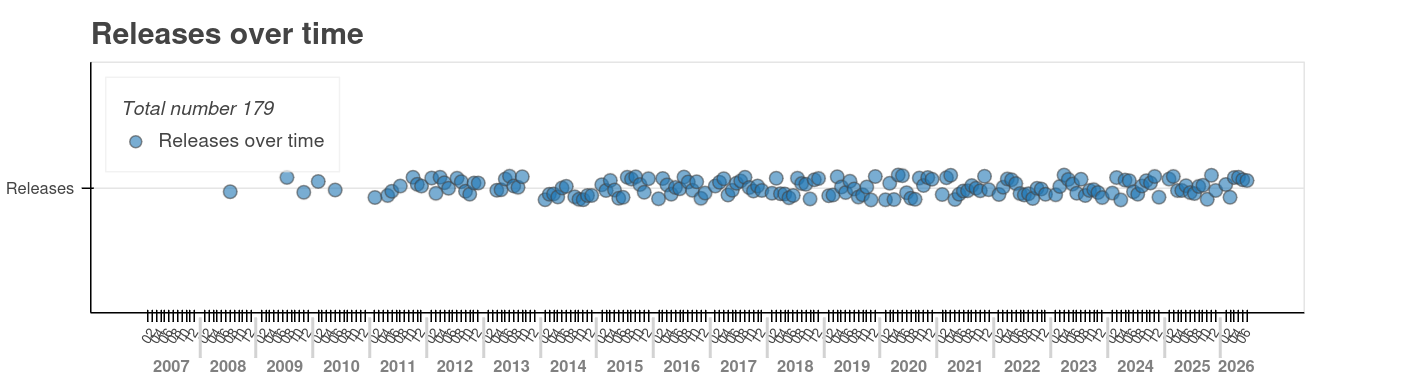
\includegraphics[width=0.99\linewidth]{./img/misp-releases.png}
    \end{center}
\end{frame}

\begin{frame}
    \frametitle{What is MISP?}
    \begin{itemize}
        \item Used worldwide to \textbf{manage and share threat-related information and intelligence}.
        \item \textbf{Open-Source Commitment}: Users of MISP can rely on the tool remaining open source and never becoming closed source (autonomy of the users).
    \end{itemize}

    \begin{center}
        
\includegraphics[width=0.99\linewidth]{./img/contributors.png}
        \vspace{0.1em}
        \scriptsize \texttt{Number recorded on March 2026}
    \end{center}
\end{frame}

\begin{frame}
    \frametitle{What is MISP?}
    \begin{itemize}
        \item A tool that {\bf collects} from partners, your analysts, your tools, feeds, $\cdots$
        \item Normalises, {\bf correlates}, {\bf enriches} the data
        \item Allows teams and communities to {\bf collaborate} and {\bf share}
        \item {\bf Feeds} automated protective tools and {\bf disseminate}
    \end{itemize}
\end{frame}

\begin{frame}
    \frametitle{Who is Using MISP?}
    \vspace{-1em}
    \textbf{Communities:} Groups of users sharing within a set of common objectives and values.
    \vspace{1em}

    \begin{columns}[T]
    \begin{column}{0.5\textwidth}
        \begin{itemize}
            \item \textbf{Private Sector}
                \vspace{-0.2em}
                \begin{itemize}
                    \item[] Financial, telecom, manufacturing
                \end{itemize}
                % \vspace{0.1em}
            \item \textbf{Military Organizations}
                \vspace{-0.2em}
                \begin{itemize}
                    \item[] Military and governmental CERT
                \end{itemize}
                % \vspace{0.1em}
            \item \textbf{Security Vendors}
                \vspace{-0.2em}
                \begin{itemize}
                    \item[] Vendor-led intelligence sharing
                \end{itemize}
                % \vspace{0.1em}
            \item \textbf{ISACs}
            \item \textbf{Trusted Groups}
                \vspace{-0.2em}
                \begin{itemize}
                    \item[] Inc. air-gapped trusted sharing
                \end{itemize}
                % \vspace{0.1em}
            \item \textbf{Law Enforcement Agencies}
            \item \textbf{International Groups}
        \end{itemize}
    \end{column}
    \hfill
    \begin{column}{0.5\textwidth}
        \centering
        \hfil
        
\includegraphics[width=\linewidth, keepaspectratio]{./img/org-count-misppriv.png}
        \vspace{0.1em}
        \scriptsize \texttt{Aggregated from misppriv.circl.lu (June 2026)}
    \end{column}
    \end{columns}

\end{frame}

\begin{frame}
    \frametitle{MISP and Threat Intelligence}
    \vspace{-1em}
    MISP is designed from the ground up to perform \textbf{context-rich threat intelligence}
    \vspace{1em}

    \begin{columns}[T]
    \begin{column}{0.55\textwidth}
        \begin{itemize}
            \item {\bf Enrich} information with context and metadata
            \item Maps {\bf Threats and TTPs}
                \vspace{-0.2em}
                \begin{itemize}
                    \item[] {\small e.g MITRE ATT\&CK}
                \end{itemize}
                \vspace{0.1em}
            \item Supports many {\bf standardized classification} marking
            \item Enables information {\bf curation} through automated quality checks
            \item Generates customizable {\bf threat reports}
            \item Allows creation of {\bf Dashboard} for trend analysis
        \end{itemize}
    \end{column}
    \hfill
    \begin{column}{0.45\textwidth}
        \centering
        \hfil
        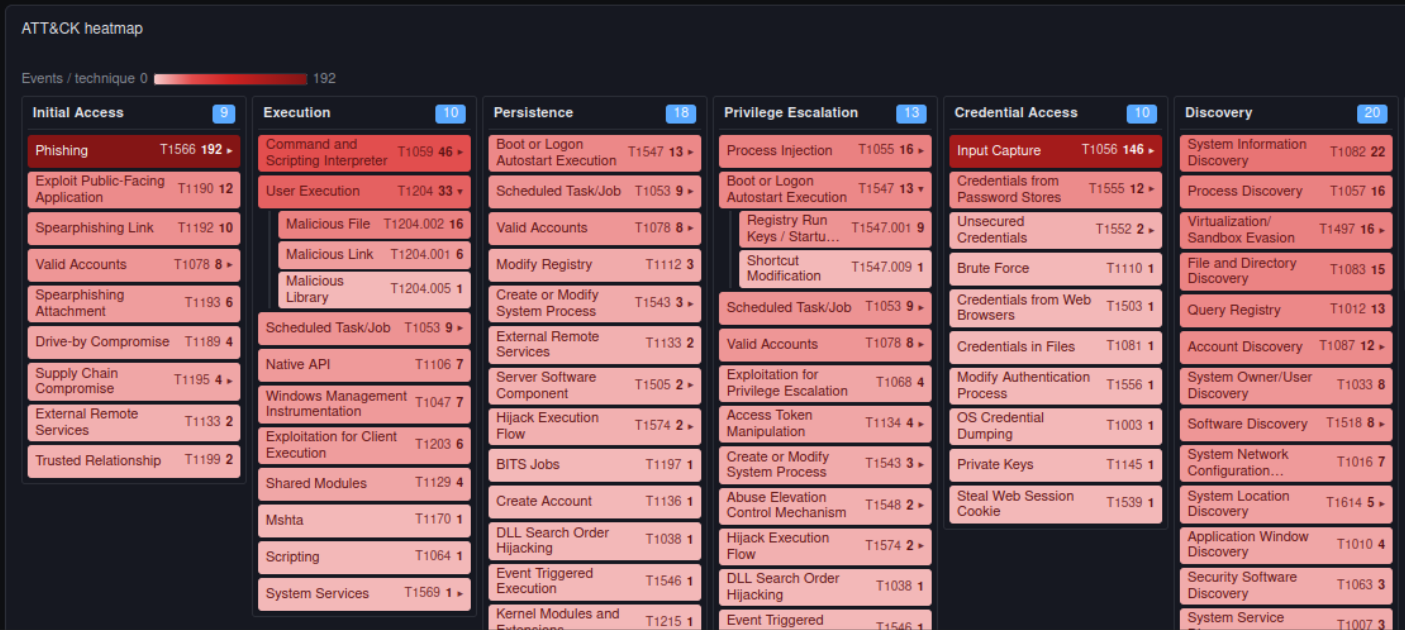
\includegraphics[width=\linewidth, keepaspectratio]{./img/misp-ttps.png}
        \vspace{0.1em}
        \scriptsize \texttt{MITRE ATT\&CK Matrix}
    \end{column}
    \end{columns}
\end{frame}

\begin{frame}
    \frametitle{Information Quality Management}

    MISP provides mechanisms to maintain, enrich and operationalize intelligence throughout its lifecycle.

    \begin{center}
        \begin{columns}[T]
            \begin{column}{0.6\textwidth}
                \card{\linewidth}{1.5em}{\faCheckCircle \, \textbf{Data Quality}}
                    {
                        {\setlength{\leftmargini}{1.0em}
                        \begin{itemize}
                            \item False Positive Management \& Feedback Loops
                            \item Knowledge Base and Vocabularies\\
                                \hspace{1em}{$\triangleright$ \, \small \textit{Address the Who, What, How and Why.}}
                        \end{itemize}
                        }
                    }
            \end{column}
            \hfill
            \begin{column}{0.4\textwidth}
                \card{\linewidth}{1.5em}{\faMagic \, \textbf{Enrichment}}
                    {
                        {\setlength{\leftmargini}{1.0em}
                        \begin{itemize}
                            \item Enrichment system
                            \item Multiple Correlation types\\
                                \hspace{1em}{\small Raw, Fuzzy Hash, CDIR}
                        \end{itemize}
                        }
                    }
            \end{column}
        \end{columns}
        % \vspace{0.5em}
        \begin{columns}[T]
            \begin{column}{0.5\textwidth}
                \card{\linewidth}{1.5em}{\faGavel \, \textbf{Governance}}
                    {
                        {\setlength{\leftmargini}{1.0em}
                        \begin{itemize}
                            \item Review Workflows
                            \item Publication Control
                            \item Lifecycle Management
                        \end{itemize}
                        }
                    }
            \end{column}
            \hfill
            \begin{column}{0.5\textwidth}
                \card{\linewidth}{1.5em}{\faLink \, \textbf{Integration}}
                    {
                        {\setlength{\leftmargini}{1.0em}
                        \begin{itemize}
                            \item API \& Automation ecosystem
                            \item Integration with External Tools
                            \item Notebooks
                        \end{itemize}
                        }
                    }
            \end{column}
        \end{columns}
    \end{center}
\end{frame}

\begin{frame}
    \frametitle{Flexible Data Format}

    \begin{center}
        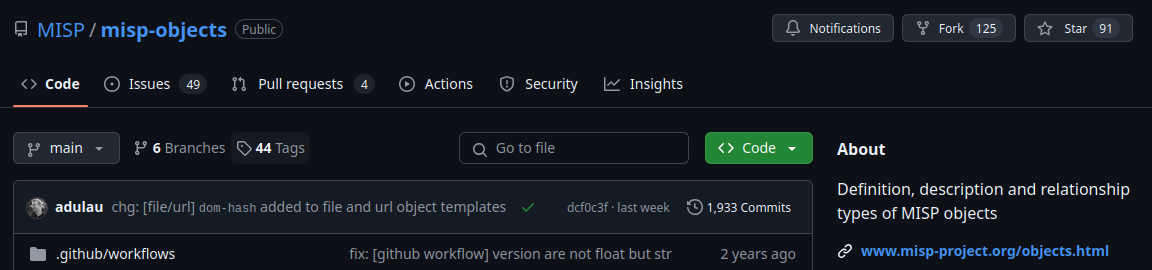
\includegraphics[width=0.8\linewidth]{./img/misp-objects-repo.png}
    \end{center}

    % \vspace{0.3em}
    \begin{center}
        \small
        MISP Objects provide reusable templates to model virtually any investigative artifact.
    \end{center}
    \vspace{0.1em}

    \centering

       \begin{center}
        \begin{columns}[T]
            \begin{column}{0.33\textwidth}
                \card{\linewidth}{1.5em}{\faGlobe \, \textbf{Network}}
                    {IPs, URLs, hashes}
            \end{column}
            \hfill
            \begin{column}{0.33\textwidth}
                \card{\linewidth}{1.5em}{\faLaptop \, \textbf{Devices}}
                    {Phones, software}
            \end{column}
            \begin{column}{0.33\textwidth}
                \card{\linewidth}{1.5em}{\faCreditCard \, \textbf{Payments}}
                    {Cards, transactions, crypto}
            \end{column}
        \end{columns}
        % \vspace{0.5em}
        \begin{columns}[T]
             \begin{column}{0.33\textwidth}
                \card{\linewidth}{1.5em}{\faCar \, \textbf{Vehicles}}
                    {Cars, aircraft, drones}
            \end{column}
            \hfill
            \begin{column}{0.33\textwidth}
                \card{\linewidth}{1.5em}{\faIdCard \, \textbf{Identities}}
                    {Persons, passports, PNR}
            \end{column}
            \begin{column}{0.33\textwidth}
                \card{\linewidth}{1.5em}{\faPuzzlePiece \, \textbf{Extensible...}}
                    {420+ Templates}
            \end{column}
        \end{columns}
    \end{center}

\end{frame}

\begin{frame}
    \frametitle{Rich Marking and Knowledge Base}

    \begin{columns}[T,onlytextwidth]
        \column{0.5\textwidth}
        \begin{itemize}
            \item \textbf{Typical CTI}
            \begin{itemize}
                \item Threat Actors
                \item Countries
                \item Attack Techniques
                \item Campaigns
                \item And \textbf{many more} $\cdots$
            \end{itemize}
        \end{itemize}

        \vspace{0.5em}

        \begin{itemize}
            \item \textbf{Impact}
            \begin{itemize}
                \item Geographical / Sectorial
                \item Demographical
                \item Economical / Legal / Regulatory
                \item Assets / Users
                \item Affected availabilities / Data Integrity
            \end{itemize}
        \end{itemize}

        \column{0.5\textwidth}

        \begin{itemize}
            \item \textbf{Confidentiality}
            \begin{itemize}
                \item Copyrighted / Classified
                \item Disclosure
            \end{itemize}
        \end{itemize}

        \vspace{0.5em}

        \begin{itemize}
            \item \textbf{Responsibility}
            \begin{itemize}
                \item Governance - 3rd party Hosted
                \item Management / Ownership
                \item Confidence / Estimative Language
                \item Discovery
            \end{itemize}
        \end{itemize}

        \vspace{0.5em}

        \begin{itemize}
            \item \textbf{Extensible} $\cdots$
            \begin{itemize}
                \item {350+ Different Vocabularies}
            \end{itemize}
        \end{itemize}

    \end{columns}
\end{frame}


\begin{frame}
    \frametitle{Using the Power of the Community}

    MISP provides multiple mechanisms to foster collaboration between analysts, teams and communities.

    % \vspace{1em}

    \begin{center}

        \begin{columns}[T]

            \begin{column}{0.49\textwidth}
                \card{\linewidth}{2.5em}
                    {{\Large\faUsers}\hspace{0.3em}\textbf{Collaboration}}
                    {
                        \begin{itemize}
                            \item Proposals
                            \item Sightings
                            \item Extended Events
                        \end{itemize}
                    }
            \end{column}

            \begin{column}{0.49\textwidth}
                \card{\linewidth}{2.5em}
                    {{\Large\faComments}\hspace{0.3em}\textbf{Discussion}}
                    {
                        \begin{itemize}
                            \item Analyst Notes
                            \item Opinions
                        \end{itemize}
                    }
            \end{column}

        \end{columns}

        \vspace{-0.5em}
        \centering
        \begin{columns}[T]

            \begin{column}{0.6\textwidth}
            \card{1.0\linewidth}{2.5em}
                {{\Large\faGlobe}\hspace{0.3em}\textbf{Specialized Sharing}}
                {
                    \begin{itemize}
                        \item Delegation
                        \item Sharing Groups
                        \item Trust Communities
                    \end{itemize}
                }
                \end{column}

        \end{columns}
    \end{center}

    \vspace{1em}

    \centering
    \small
    Collaboration can happen within a team, across organizations, or through trusted sharing communities.

\end{frame}
